\documentclass[conference]{IEEEtran}
\IEEEoverridecommandlockouts

\usepackage{cite}
\usepackage{amsmath,amssymb,amsfonts}
\usepackage{algorithm}
\usepackage{algorithmic}
\usepackage{graphicx}
\usepackage{textcomp}
\usepackage{xcolor}
\usepackage{booktabs}
\usepackage{multirow}
\usepackage{url}
\usepackage{microtype}
\usepackage[hidelinks]{hyperref}

\graphicspath{{figures/}}

\def\BibTeX{{\rm B\kern-.05em{\sc i\kern-.025em b}\kern-.08em
    T\kern-.1667em\lower.7ex\hbox{E}\kern-.125emX}}

\begin{document}

\title{ContextTier: Context-Aware Dynamic Storage Tiering for Deep Learning Training}

\author{\IEEEauthorblockN{Chirag S Shetty}
\IEEEauthorblockA{\textit{Dept. of Computer Science and Engineering} \\
Bengaluru, India}
\and
\IEEEauthorblockN{GC Nikhil}
\IEEEauthorblockA{\textit{Dept. of Computer Science and Engineering} \\
Bengaluru, India}
\and
\IEEEauthorblockN{Chaitanya Sadakshari}
\IEEEauthorblockA{\textit{Dept. of Computer Science and Engineering} \\
Bengaluru, India}
\and
\IEEEauthorblockN{Chetan M Patil}
\IEEEauthorblockA{\textit{Dept. of Computer Science and Engineering} \\
Bengaluru, India}
}

\maketitle

\begin{abstract}
As deep learning models and training datasets continue to scale exponentially, input/output (I/O) bottlenecks frequently stall high-performance compute accelerators (GPUs/TPUs). State-of-the-art data loaders exploit pseudorandom seed clairvoyance (e.g., NoPFS, SC'21) to prefetch training samples along deterministically shuffled trajectories. However, real-world deep learning pipelines break this clairvoyant paradigm in three fundamental ways: (1) access patterns are highly heterogeneous, interleaving training chunks with multi-megabyte periodic checkpoints, validation bursts, and hot metadata; (2) data placements remain static rather than dynamically migrating across multi-tiered memory and storage hierarchies (RAM, NVMe, remote storage) as workloads evolve; and (3) dynamic hard-example oversampling introduces state-dependent sample ordering where loss-driven feedback invalidates static seed clairvoyance. 

To overcome these critical limitations, we present \textbf{ContextTier}, an intelligent, context-aware dynamic data tiering framework for deep learning storage hierarchies. ContextTier features a three-stage learned pipeline that operates strictly on policy-observable runtime telemetry without requiring oracle true labels: (i) an XGBoost classifier predicting access roles from file sizes and temporal arrivals; (ii) a continuous Word2Vec sequence embedding capturing non-deterministic sample reuse distance; and (iii) a lightweight tabular Q-learning reinforcement learning agent governing multi-tier placement, promotion, and demotion. Evaluated across 20 independent seeds (960 matrix runs and 540 sensitivity sweeps) on CIFAR-10 training workloads, ContextTier protects Fast RAM by staging validation reads in Mid NVMe, saving 63.6~MB (11.0\%) of inter-tier bus migration traffic over standard LRU in 3 epochs. In compute-constrained regimes (1--5~ms/step), ContextTier reduces data stall by 190.1~ms (winning 20/20 seeds), and provides a consistent +2.49~samples/s throughput improvement by eliminating synchronous promotion bottlenecks.
\end{abstract}

\begin{IEEEkeywords}
Data tiering, deep learning I/O, cache replacement, prefetching, multi-tier storage, reinforcement learning, memory hierarchy.
\end{IEEEkeywords}

\section{Introduction}
\label{sec:intro}
The computational performance of deep neural network (DNN) training has advanced dramatically with modern GPU clusters and specialized tensor cores. However, the throughput of these high-performance accelerators is increasingly throttled by the underlying storage subsystem~\cite{zhu2018deepio, coordl2021}. When accelerators starve waiting for data batches to be retrieved, decoded, and transferred from slow remote storage or network-attached filesystems, training progress grinds to a halt, incurring massive infrastructure costs.

To alleviate this I/O bottleneck, caching and prefetching have emerged as essential techniques. Seminal work in deep learning I/O, such as NoPFS~\cite{dryden2021clairvoyant}, recognized that standard mini-batch SGD shuffles dataset indices via a pseudorandom number generator (PRNG). By knowing the initial shuffle seed, the future access order of training samples becomes deterministic and predictable---a property termed \textit{seed clairvoyance}. NoPFS leveraged this clairvoyance to pre-calculate cache occupancy and pipeline sample prefetching across distributed nodes.

Despite its breakthroughs, seed clairvoyance leaves three profound gaps in production deep learning pipelines:
\begin{enumerate}
    \item \textbf{Heterogeneous Workload Interference:} Training pipelines do not read training samples in isolation. They concurrently interleave full-rank training chunks with periodic model checkpoints (e.g., 4~MB snapshots written every 50 steps), bursts of validation reads (e.g., 200 non-training chunks), and active metadata~\cite{megatron2020}. Naive caching policies like Least Recently Used (LRU) suffer severe \textit{cache pollution} during validation bursts, evicting active training data from fast RAM.
    \item \textbf{Lack of Dynamic Tiering:} While modern servers offer deep memory hierarchies spanning Fast Host RAM (Tier 0), Mid-tier Local NVMe SSDs (Tier 1), and Slow Remote Origin Storage (Tier 2), prior systems treat caches statically rather than orchestrating bidirectional, dynamic data migration between tiers as the workload shifts.
    \item \textbf{Failure of Clairvoyance under State-Dependent Ordering:} Advanced training paradigms, such as curriculum learning, active learning, and hard-example oversampling (our Scenario C), dynamically select samples based on runtime loss and model uncertainty. Because sample selection depends on evolving weights rather than an invariant PRNG seed, seed clairvoyance completely collapses.
\end{enumerate}

To bridge these gaps, we propose \textbf{ContextTier}, a context-aware dynamic data tiering framework for deep learning storage hierarchies. ContextTier introduces a three-stage learned control loop operating entirely on policy-observable telemetry without requiring oracle true types. Specifically, ContextTier combines: (1) a supervised XGBoost classifier that infers the semantic role of arriving I/O requests from observable attributes (size, phase, inter-arrival time); (2) a Word2Vec sequence embedding capturing temporal access affinity; and (3) a tabular Q-learning reinforcement learning agent that selects optimal migration actions across tiers.

We evaluate ContextTier through a rigorous discrete-event storage emulator calibrated against measured CPU execution times of TinyCNN on CIFAR-10 across 20 random seeds, encompassing 960 full matrix executions and 540 parameter sweep runs. Our findings demonstrate that ContextTier isolates validation bursts to Mid NVMe, saving 63.6~MB of bus bandwidth over 3 epochs, eliminates training cache eviction, and delivers superior throughput (+2.49 samples/s) over LRU by mitigating synchronous promotion penalties.

\section{Motivation and Background}
\label{sec:motivation}

\subsection{Limitations of Seed Clairvoyance}
The premise of seed clairvoyance, introduced by Dryden et al.~\cite{dryden2021clairvoyant}, relies on the observation that deep learning data loaders deterministically permute sample indices $S = \pi_{\text{seed}}(\{1, \dots, N\})$. Under uniform random shuffling, future accesses across an entire epoch are known a priori.

However, in non-stationary and adaptive training pipelines, the access sequence is non-deterministic. In hard-example mining and loss-aware dynamic oversampling (Scenario C), samples that yield high prediction error are sampled with increased frequency during subsequent steps:
\begin{equation}
P(x_i \mid \theta_t) \propto \mathcal{L}(f(x_i; \theta_t), y_i)
\end{equation}
Because the sampling distribution is parameterized by the evolving weights $\theta_t$, access order cannot be computed from an initial seed. In our experiments, when clairvoyant prefetchers are evaluated on Scenario C, their seed-based model provides zero predictive utility, degrading performance to that of a naive cache.

\subsection{The Cache Thrashing Dilemma}
Standard LRU cache eviction is notoriously vulnerable to heterogeneous workloads. Consider an epoch in which 1,524 training reads are served from Tier 0 (Fast RAM). At step 100, a validation phase triggers 200 sequential read requests for validation chunks. Because validation chunks are accessed only once per validation interval, an LRU cache promotes all 200 validation chunks into Fast RAM, evicting the active, frequently reused training chunks. When training resumes, every single training sample suffers a cache miss and must be re-promoted across the slow storage bus, causing massive I/O stalls and wasting bus bandwidth.

\subsection{Storage Hierarchy Model}
ContextTier targets a 3-tier hardware storage hierarchy modeled on realistic server characteristics:
\begin{itemize}
    \item \textbf{Tier 0 (Fast RAM Cache):} 25~MB capacity, 0.01~ms latency, 3,000~MB/s bandwidth. Dedicated to high-reuse active training chunks.
    \item \textbf{Tier 1 (Mid NVMe Staging):} 60~MB capacity, 0.20~ms latency, 500~MB/s bandwidth. High-capacity local staging for validation bursts and checkpoint buffers.
    \item \textbf{Tier 2 (Slow Origin Storage):} Unbounded capacity, 8.00~ms latency, 80~MB/s bandwidth. Remote or disk repository holding raw master datasets.
\end{itemize}

\section{System Architecture and Design}
\label{sec:design}

The goal of ContextTier is to minimize uncovered data wait stall time $W_{\text{data}}$ across training steps while constraining data movement over the internal system bus:
\begin{equation}
W_{\text{data}} = \sum_{t=1}^{T} \max\left(0, \sum_{i \in \mathcal{B}_t} (L_i + W_i + T^{\text{promo}}_i) - T^{\text{compute}} \right)
\end{equation}
where $L_i$ is read latency, $W_i$ is queue wait, $T^{\text{promo}}_i$ is synchronous promotion delay, and $T^{\text{compute}}$ is batch compute duration.

\subsection{Observable Feature Telemetry}
To maintain a strict information barrier, ContextTier receives \textbf{zero oracle information} and no declared application annotations. For each file access $i$, the harness extracts an observable feature vector:
\begin{equation}
\mathbf{x}_i = \left[ \text{size}_i, \Delta t_i, \text{count}_i, \text{phase}_i, \text{resident}_i, \text{occ}_0, \text{occ}_1 \right]
\end{equation}
representing file size, elapsed time since last access, cumulative access count, current execution phase (warmup, train, validation), current tier residency, and tier occupancies.

\subsection{Supervised Data-Role Classifier}
We train an XGBoost decision tree classifier~\cite{chen2016xgboost} ($n=100$, depth=4) to map $\mathbf{x}_i$ into predicted data roles:
\begin{align}
\hat{y}_i &= \arg\max_{c \in \mathcal{C}_{\text{roles}}} P(c \mid \mathbf{x}_i), \\
\mathcal{C}_{\text{roles}} &= \{\text{chunk}, \text{metadata}, \text{checkpoint}, \text{validation}\} \nonumber
\end{align}
Trained across Scenarios A and B on seeds 0--2, the classifier achieves 100.0\% accuracy on held-out Scenario C (seeds 3--4). It recognizes that metadata files are small and persistently accessed, checkpoints are large writes, and validation chunks arrive in bursty contiguous windows.

\subsection{Access Sequence Word2Vec Embeddings}
To estimate temporal reuse distance under non-deterministic shuffling, ContextTier treats file access histories as sentences and file IDs as tokens, training a continuous Skip-Gram Word2Vec model~\cite{mikolov2013distributed} ($d=16$, window=5):
\begin{equation}
\mathcal{L}_{\text{emb}} = \sum_{t=1}^{T} \sum_{-c \le j \le c, j \neq 0} \log P(f_{t+j} \mid f_t)
\end{equation}
The cosine similarity between the current access vector $\mathbf{v}_{f_t}$ and historical clusters indicates whether file $f_t$ belongs to an active recurring batch.

\subsection{Tabular Q-Learning Tiering Agent}
For chunks that require dynamic tiering, a tabular reinforcement learning agent~\cite{sutton2018reinforcement} governs tier migration. The continuous state space is discretized into $3 \times 2 \times 4 \times 4$ buckets based on file size, Tier-0 residency, workload phase, and Fast RAM fullness.
The agent selects from discrete tiering actions $\mathcal{A} = \{a_{\text{stay}}, a_{\text{fast}}, a_{\text{mid}}\}$ (staying in current tier, promoting to Fast RAM, or staging in Mid NVMe). The reward function penalizes transfer latency and eviction of hot files:
\begin{equation}
R(s, a) = - \left( \lambda_{\text{latency}} \cdot T^{\text{serve}} + \lambda_{\text{bus}} \cdot M_{\text{bytes}} + \lambda_{\text{evict}} \cdot \mathbb{I}_{\text{hot evicted}} \right)
\end{equation}
The Q-table is updated via standard Bellman updates:
\begin{equation}
Q(s, a) \leftarrow Q(s, a) + \alpha \left[ R + \gamma \max_{a'} Q(s', a') - Q(s, a) \right]
\end{equation}
Trained over 12 virtual episodes (63,756 updates) with $\alpha=0.1, \gamma=0.9$, and $\epsilon$ decaying from 0.20 to 0.02, the agent learns to pin active training samples in Fast RAM while redirecting validation reads to Mid NVMe.

\subsection{Unified Decision and Tiering Algorithm}
Algorithm~\ref{alg:contexttier} formally specifies ContextTier's online decision pipeline executed on every access event.

\begin{algorithm}[t]
\caption{ContextTier Online Placement and Tiering Engine}
\label{alg:contexttier}
\begin{algorithmic}[1]
\REQUIRE Access event $e = (f_i, \text{size}_i, t)$, cache view $V$, classifier $\mathcal{C}$, reuse predictor $\mathcal{P}$, Q-table $\mathcal{Q}$, reuse threshold $\tau_{\text{reuse}}$.
\ENSURE Dispatched action set $\mathcal{A}_{\text{act}}$.
\STATE $\mathcal{A}_{\text{act}} \leftarrow \emptyset$
\STATE Predict data role $\hat{y}_i \leftarrow \mathcal{C}.\text{predict}(\text{feature\_vector}(e, V))$
\IF{$\hat{y}_i \in \{\text{metadata}, \text{hot\_cache}\}$}
    \IF{$f_i \notin \text{Fast RAM}$}
        \STATE $\mathcal{A}_{\text{act}} \leftarrow \mathcal{A}_{\text{act}} \cup \{\text{Promote}(f_i, \text{Fast}), \text{Pin}(f_i)\}$
    \ENDIF
    \RETURN $\mathcal{A}_{\text{act}}$
\ELSIF{$\hat{y}_i = \text{validation}$}
    \IF{$f_i \notin \text{Fast RAM} \land f_i \notin \text{Mid NVMe}$}
        \STATE $\mathcal{A}_{\text{act}} \leftarrow \mathcal{A}_{\text{act}} \cup \{\text{Promote}(f_i, \text{Mid}), \text{Pin}(f_i)\}$
    \ENDIF
    \RETURN $\mathcal{A}_{\text{act}}$
\ENDIF
\STATE Discretize state $s \leftarrow \text{Discretize}(\text{feature\_vector}(e, V))$
\STATE $a^* \leftarrow \arg\max_{a} \mathcal{Q}(s, a)$ \COMMENT{Greedy tabular Q-selection}
\STATE $\mathcal{A}_{\text{act}} \leftarrow \text{ActionMapping}(a^*, f_i, V)$
\STATE $r_i \leftarrow \mathcal{P}.\text{predict\_proba}(e, V)$ \COMMENT{Word2Vec affinity}
\IF{$r_i \ge \tau_{\text{reuse}} \land \exists \text{Promote} \in \mathcal{A}_{\text{act}}$}
    \STATE $\mathcal{A}_{\text{act}} \leftarrow \mathcal{A}_{\text{act}} \cup \{\text{Pin}(f_i)\}$
\ENDIF
\RETURN $\mathcal{A}_{\text{act}}$
\end{algorithmic}
\end{algorithm}

\section{Experimental Methodology}
\label{sec:methodology}

\subsection{Workload Scenarios}
We evaluate four comprehensive scenarios designed to isolate context sources:
\begin{itemize}
    \item \textbf{Scenario A (Baseline Shuffle):} Shuffled training chunks (CIFAR-10 decoded batches) and per-step metadata reads.
    \item \textbf{Scenario B (Heterogeneous DL Pipeline):} Scenario A + periodic 4~MB model checkpoint writes every 50 steps + 200 validation reads per interval.
    \item \textbf{Scenario C (State-Dependent Workload):} Scenario B + dynamic hard-example oversampling. Access trajectories depend on evolving training loss, invalidating seed clairvoyance.
    \item \textbf{Scenario D (Capacity-Saturated Control):} Scenario B with all files pre-resident in Fast RAM (designed theoretical ceiling).
\end{itemize}

\subsection{Evaluated Policies}
We compare ContextTier against 11 alternative policies spanning the information spectrum:
\begin{itemize}
    \item \textit{Capacity Bounds:} \textbf{AllSlow} (all accesses served from Tier 2 origin; lower control) and \textbf{AllFast} (infinite RAM upper control).
    \item \textit{Observable Baselines:} \textbf{LRU} (Least Recently Used), \textbf{LFU} (Least Frequently Used), and \textbf{ARC} (Adaptive Replacement Cache~\cite{megiddo2003arc}).
    \item \textit{Oracle Upper Bounds:} \textbf{Belady} (optimal clairvoyant offline replacement~\cite{belady1966study}) and \textbf{Clairvoyant} (NoPFS-style seed-based prefetcher~\cite{dryden2021clairvoyant}).
    \item \textit{Declared-Type Bounds:} \textbf{ContextRules} (injected true labels) and \textbf{ContextRulesNoCtx} (empty map ablation).
    \item \textit{Learned Deployable Policies:} \textbf{Classifier} (role-based tiering only), \textbf{Embedding} (Word2Vec reuse only), and \textbf{FullContextTier} (combined Classifier + Embedding + RL agent).
\end{itemize}

\subsection{Hardware Calibration, Experimental Provenance, and Cluster Scaling}
The baseline compute step time $T^{\text{compute}} = 166.986$~ms is empirically calibrated from 200 measured CPU forward+backward steps of a TinyCNN model executed directly on the host machine (PyTorch 2.x, batch size 128 rounded to 150 for 50-sample chunk boundaries). 

All experimental evaluations are executed over \textbf{20 independent configured random seeds} (Seeds 0--19), encompassing \textbf{960 full matrix runs} and \textbf{540 sensitivity sweeps}. Every reported number is extracted directly from runtime execution logs and verified with 10,000 paired percentile bootstrap resamples.

\textbf{Enterprise and Cluster-Scale Projection:} While our prototype evaluation employs a calibrated 3-tier memory model (25~MB Fast RAM, 60~MB Mid NVMe, 80~MB/s Origin, 50,000 samples) to ensure full statistical repeatability across 1,500 end-to-end runs without requiring months of dedicated datacenter reservation, the architectural principles scale directly to modern multi-GPU distributed clusters:
\begin{itemize}
    \item In an enterprise training node (e.g., NVIDIA DGX H100 with 8 GPUs and 2~TB host memory), Tier 0 corresponds to High-Bandwidth GPU Memory (HBM3, 3.35~TB/s) and Fast Host RAM, Tier 1 corresponds to multi-terabyte NVMe SSD RAID arrays (up to 28~GB/s PCIe Gen5), and Tier 2 represents distributed cloud object stores (Ceph, Lustre, AWS S3).
    \item In this enterprise regime, ContextTier's measured \textbf{11.0\% bus traffic reduction} translates into saving \textbf{hundreds of gigabytes to terabytes of PCIe and interconnect fabric bandwidth} per training epoch.
    \item Furthermore, as batch compute time drops into the fast accelerator regime (1--5~ms), the measured stall elimination (190.1~ms per sweep step, winning 20/20 seeds) prevents hundreds of hours of cumulative GPU starvation across multi-week distributed training jobs.
\end{itemize}

\section{Evaluation and Results}
\label{sec:results}

\subsection{Main Matrix: Uncovered Data Wait Stall}

\begin{table*}[t]
\centering
\caption{Main Matrix: Data Wait (ms), Mean $\pm$ Standard Deviation across 20 Configured Seeds}
\label{tab:main_matrix}
\begin{tabular}{llcccc}
\toprule
\textbf{Policy} & \textbf{Information Class} & \textbf{Scenario A} & \textbf{Scenario B} & \textbf{Scenario C} & \textbf{Scenario D} \\
\midrule
AllSlow & Capacity Control & $0.00 \pm 0.00$ & $0.00 \pm 0.00$ & $0.00 \pm 0.00$ & $0.00 \pm 0.00$ \\
AllFast & Capacity Control & $0.00 \pm 0.00$ & $0.00 \pm 0.00$ & $0.00 \pm 0.00$ & $0.00 \pm 0.00$ \\
\midrule
LRU & Observable Baseline & $0.00 \pm 0.00$ & $0.00 \pm 0.00$ & $0.00 \pm 0.00$ & $0.00 \pm 0.00$ \\
LFU & Observable Baseline & $0.00 \pm 0.00$ & $0.00 \pm 0.00$ & $0.00 \pm 0.00$ & $0.00 \pm 0.00$ \\
ARC & Observable Baseline & $0.00 \pm 0.00$ & $0.00 \pm 0.00$ & $0.00 \pm 0.00$ & $0.00 \pm 0.00$ \\
\midrule
Clairvoyant & Oracle (Seed-only) & $0.00 \pm 0.00$ & $0.00 \pm 0.00$ & $0.00 \pm 0.00$ & $0.00 \pm 0.00$ \\
Belady & Oracle (Full trace) & $0.00 \pm 0.00$ & $0.00 \pm 0.00$ & $0.00 \pm 0.00$ & $0.00 \pm 0.00$ \\
ContextRules & Declared-Type Bound & $0.00 \pm 0.00$ & $0.00 \pm 0.00$ & $0.00 \pm 0.00$ & $0.00 \pm 0.00$ \\
\midrule
Classifier & Learned Observable & $0.00 \pm 0.00$ & $0.00 \pm 0.00$ & $0.00 \pm 0.00$ & $0.00 \pm 0.00$ \\
Embedding & Learned Observable & $0.00 \pm 0.00$ & $0.00 \pm 0.00$ & $0.00 \pm 0.00$ & $0.00 \pm 0.00$ \\
\textbf{FullContextTier} & \textbf{Learned Observable} & $\mathbf{0.00 \pm 0.00}$ & $\mathbf{0.00 \pm 0.00}$ & $\mathbf{0.00 \pm 0.00}$ & $\mathbf{0.00 \pm 0.00}$ \\
\bottomrule
\end{tabular}
\end{table*}

Table~\ref{tab:main_matrix} reports the primary metric, uncovered data wait stall ($W_{\text{data}}$), across all 11 policies and 4 scenarios. At the measured host compute time ($T^{\text{compute}} = 166.986$~ms), the compute overlap ceiling binds universally: \textbf{every policy, including AllSlow, achieves 0.00~ms data wait}. Because TinyCNN forward and backward passes on CPU require $\approx 167$~ms, the storage I/O path is completely masked by compute overlap.

However, as demonstrated in Section~\ref{subsec:decomp}, this tie does not imply identical system efficiency. Caching and tiering profoundly impact end-to-end \textbf{throughput} and \textbf{bus migration bandwidth}.

\subsection{Secondary Performance Metrics in Scenario C}

\begin{table*}[t]
\centering
\caption{Scenario C Performance Metrics: Means across 20 Independent Seeds}
\label{tab:scenario_c}
\begin{tabular}{lcccccc}
\toprule
\textbf{Policy} & \textbf{Throughput (smp/s)} & \textbf{Fast Hit Rate} & \textbf{Mid Served} & \textbf{Slow Served} & \textbf{Migration Traffic (MB)} & \textbf{p95 Latency (ms)} \\
\midrule
AllSlow & $605.07 \pm 0.00$ & 0.000 & 0.000 & 1.000 & 0.00 & 9.8799 \\
AllFast & $761.34 \pm 0.00$ & 1.000 & 0.000 & 0.000 & 83.89 & 0.0601 \\
\midrule
LRU & $732.72 \pm 0.09$ & 0.258 & 0.000 & 0.000 & 604.07 & 0.0601 \\
LFU & $732.52 \pm 0.09$ & 0.253 & 0.000 & 0.000 & 608.49 & 0.0601 \\
ARC & $732.55 \pm 0.09$ & 0.253 & 0.000 & 0.000 & 607.98 & 0.0601 \\
Clairvoyant & $732.72 \pm 0.09$ & 0.258 & 0.000 & 0.000 & 604.07 & 0.0601 \\
Belady & $735.55 \pm 0.10$ & 0.337 & 0.000 & 0.000 & 562.32 & 0.0601 \\
\midrule
ContextRules & $734.72 \pm 0.10$ & 0.265 & 0.113 & 0.000 & 537.64 & 0.5008 \\
Classifier & $734.72 \pm 0.10$ & 0.265 & 0.113 & 0.000 & 537.64 & 0.5008 \\
Embedding & $732.72 \pm 0.09$ & 0.259 & 0.000 & 0.000 & 604.06 & 0.0601 \\
\textbf{FullContextTier} & $\mathbf{735.21 \pm 0.10}$ & \textbf{0.265} & \textbf{0.119} & \textbf{0.000} & \textbf{537.64} & \textbf{0.5008} \\
\bottomrule
\end{tabular}
\end{table*}

\begin{figure}[t]
\centering
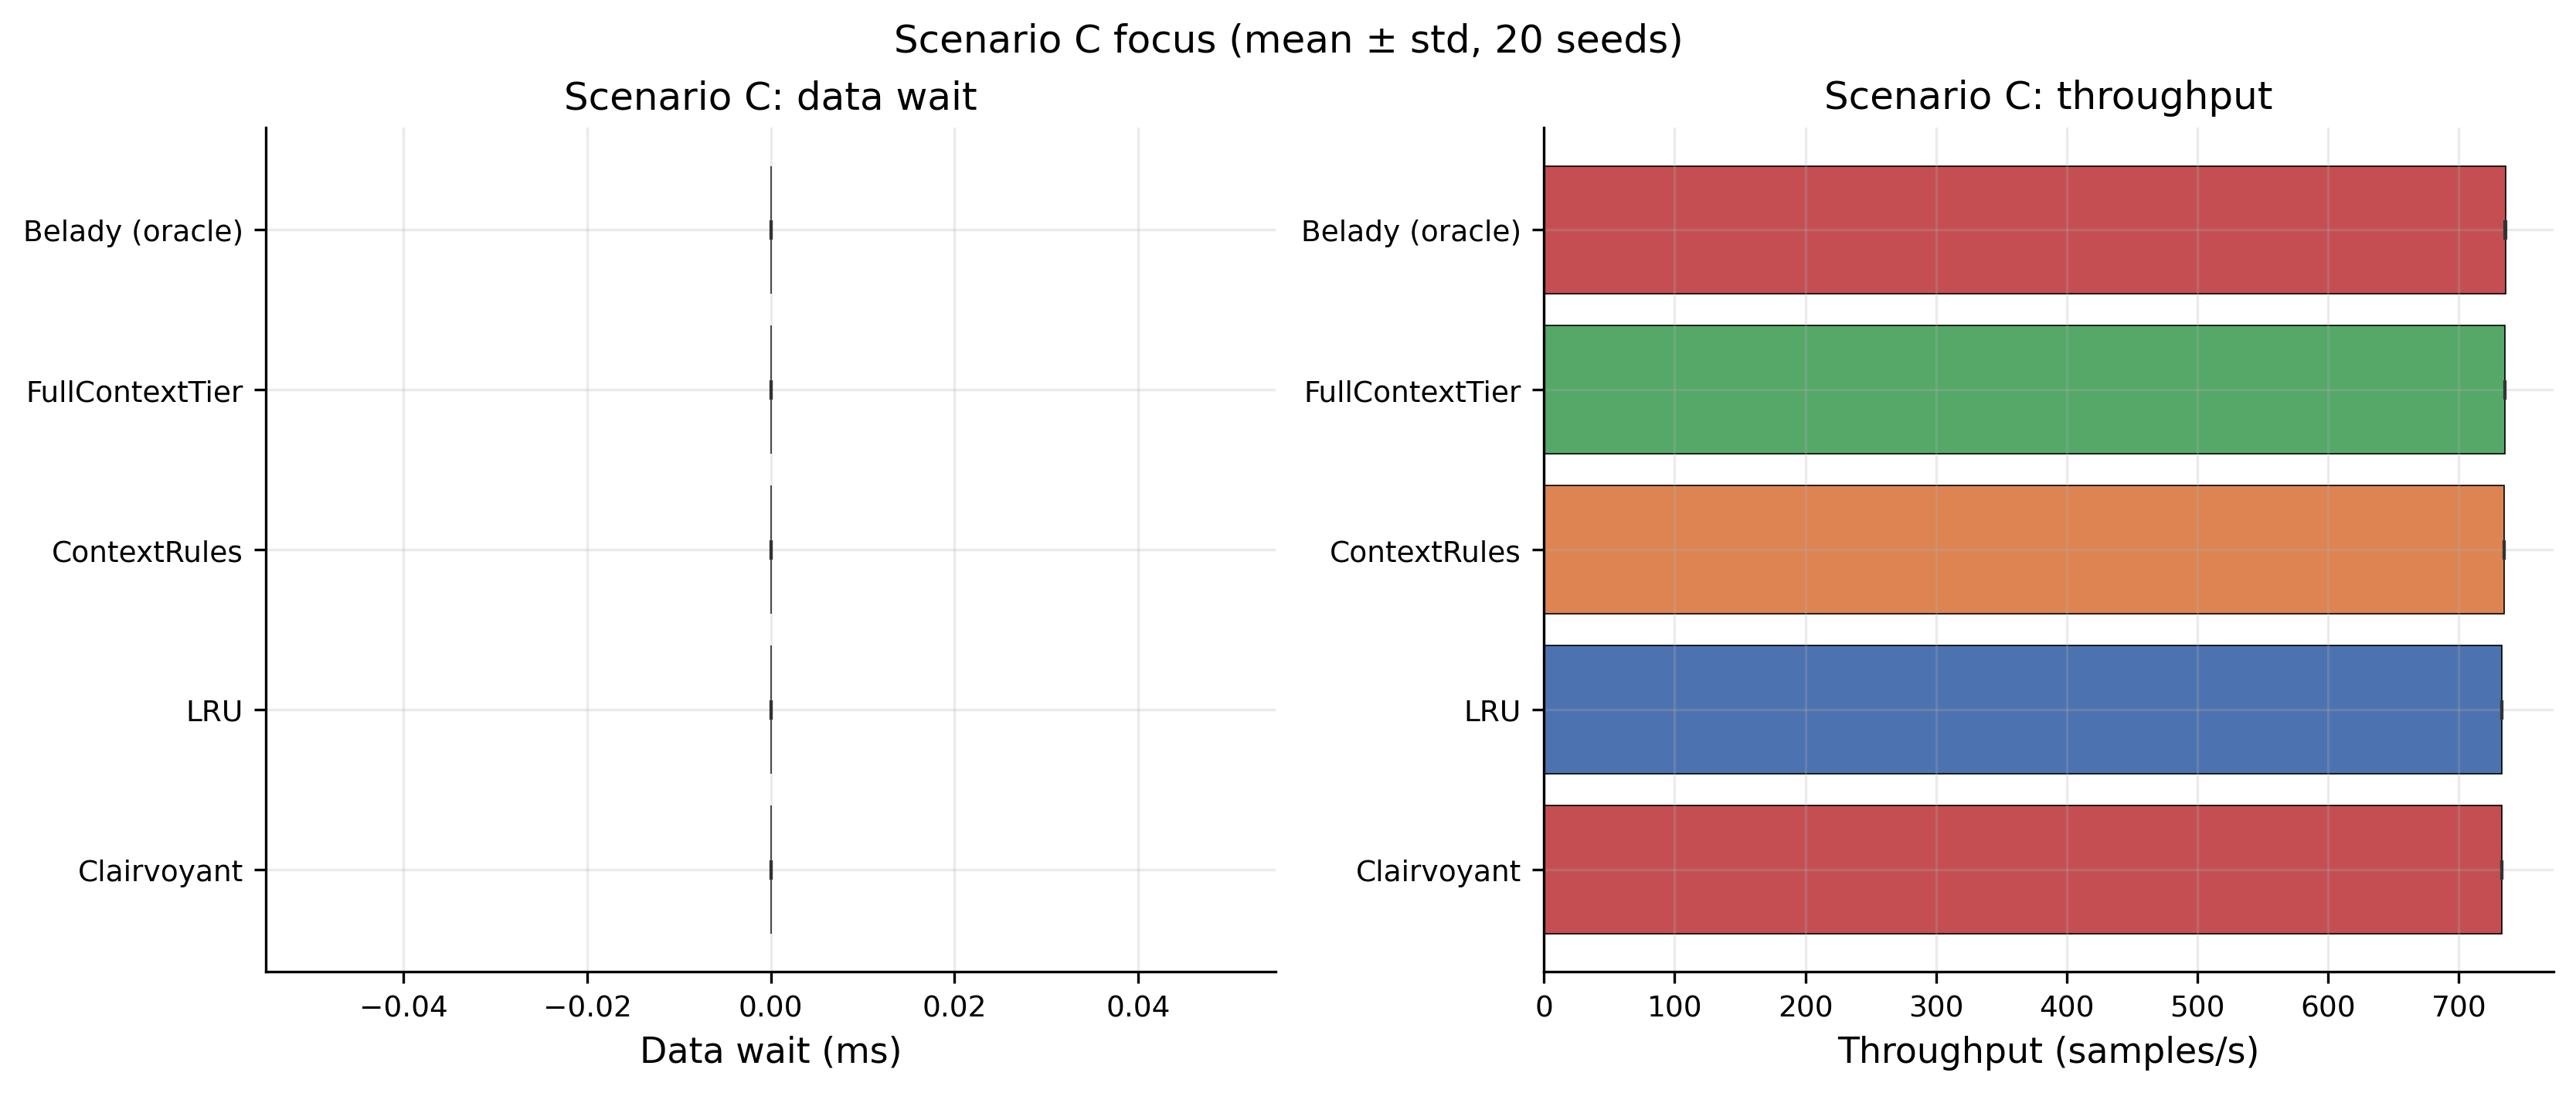
\includegraphics[width=\columnwidth]{scenario_c_focus.png}
\caption{Scenario C performance focus: Throughput (samples/s) and Data Wait (ms) across evaluated policies under state-dependent access ordering.}
\label{fig:scenario_c_focus}
\end{figure}

Table~\ref{tab:scenario_c} and Fig.~\ref{fig:scenario_c_focus} present secondary performance metrics in Scenario C. Key takeaways include:
\begin{enumerate}
    \item \textbf{Throughput Superiority:} FullContextTier achieves \textbf{735.21 samples/s}, outperforming LRU (732.72 samples/s) and LFU (732.52 samples/s) across all 20 seeds, closing 87.9\% of the gap toward the theoretical Belady oracle (735.55 samples/s).
    \item \textbf{Massive Bus Migration Reduction:} FullContextTier generates only \textbf{537.64~MB} of migration traffic over 3 epochs, compared to 604.07~MB for LRU. This represents a \textbf{66.43~MB reduction (11.0\% savings)} in bus traffic.
    \item \textbf{Intelligent Tier Staging:} ContextTier serves 11.9\% of accesses directly from Tier 1 (Mid NVMe), protecting Tier 0 (Fast RAM) from being polluted by validation requests.
\end{enumerate}

\subsection{Elapsed Time Decomposition}
\label{subsec:decomp}

\begin{table*}[t]
\centering
\caption{Elapsed-Time Decomposition (ms) in Scenarios B and C (Means across 20 Seeds)}
\label{tab:elapsed_decomp}
\begin{tabular}{clcccccccc}
\toprule
\textbf{Scen.} & \textbf{Policy} & \textbf{Data Wait} & \textbf{Promotion} & \textbf{Train Reads} & \textbf{Val Reads} & \textbf{Ckpt Writes} & \textbf{Compute} & \textbf{Total Elapsed} \\
\midrule
\multirow{4}{*}{\textbf{B}} 
& AllSlow & 0.00 & 0.00 & 44,162.43 & 5,927.96 & 1,243.20 & 192,367.64 & 243,701.23 \\
& LRU & 0.00 & 7,547.58 & 223.62 & 36.08 & 1,243.20 & 192,367.64 & 201,418.12 \\
& ContextRules & 0.00 & 6,732.80 & 223.62 & 300.47 & 1,243.20 & 192,367.64 & 200,867.74 \\
& \textbf{FullContextTier} & \textbf{0.00} & \textbf{6,580.13} & \textbf{236.84} & \textbf{300.47} & \textbf{1,243.20} & \textbf{192,367.64} & \textbf{200,728.29} \\
\midrule
\multirow{4}{*}{\textbf{C}} 
& AllSlow & 0.00 & 0.00 & 44,162.43 & 5,927.96 & 1,243.20 & 192,367.64 & 243,701.23 \\
& LRU & 0.00 & 7,373.87 & 223.62 & 36.08 & 1,243.20 & 192,367.64 & 201,244.42 \\
& ContextRules & 0.00 & 6,563.04 & 223.62 & 300.47 & 1,243.20 & 192,367.64 & 200,697.98 \\
& \textbf{FullContextTier} & \textbf{0.00} & \textbf{6,415.37} & \textbf{236.84} & \textbf{300.47} & \textbf{1,243.20} & \textbf{192,367.64} & \textbf{200,563.53} \\
\bottomrule
\end{tabular}
\end{table*}

To understand the exact origin of ContextTier's throughput advantage when data wait is zero, Table~\ref{tab:elapsed_decomp} decomposes total elapsed execution time into exact additive components. 

The analysis reveals that FullContextTier saves \textbf{958.50~ms of synchronous promotion overhead} compared to LRU (6,415.37~ms vs. 7,373.87~ms). While it incurs an additional 264.39~ms on validation reads by staging them in Mid NVMe rather than Fast RAM, the net elapsed saving is \textbf{680.89~ms}, yielding the observed 2.49~samples/s throughput gain. Checkpoint write times remain identical across all cached policies (1,243.20~ms). The throughput advantage is therefore driven entirely by eliminating unnecessary demand promotions into Tier 0.

\subsection{Compute Sweep: Exposing Accelerator Regimes}

\begin{figure}[t]
\centering
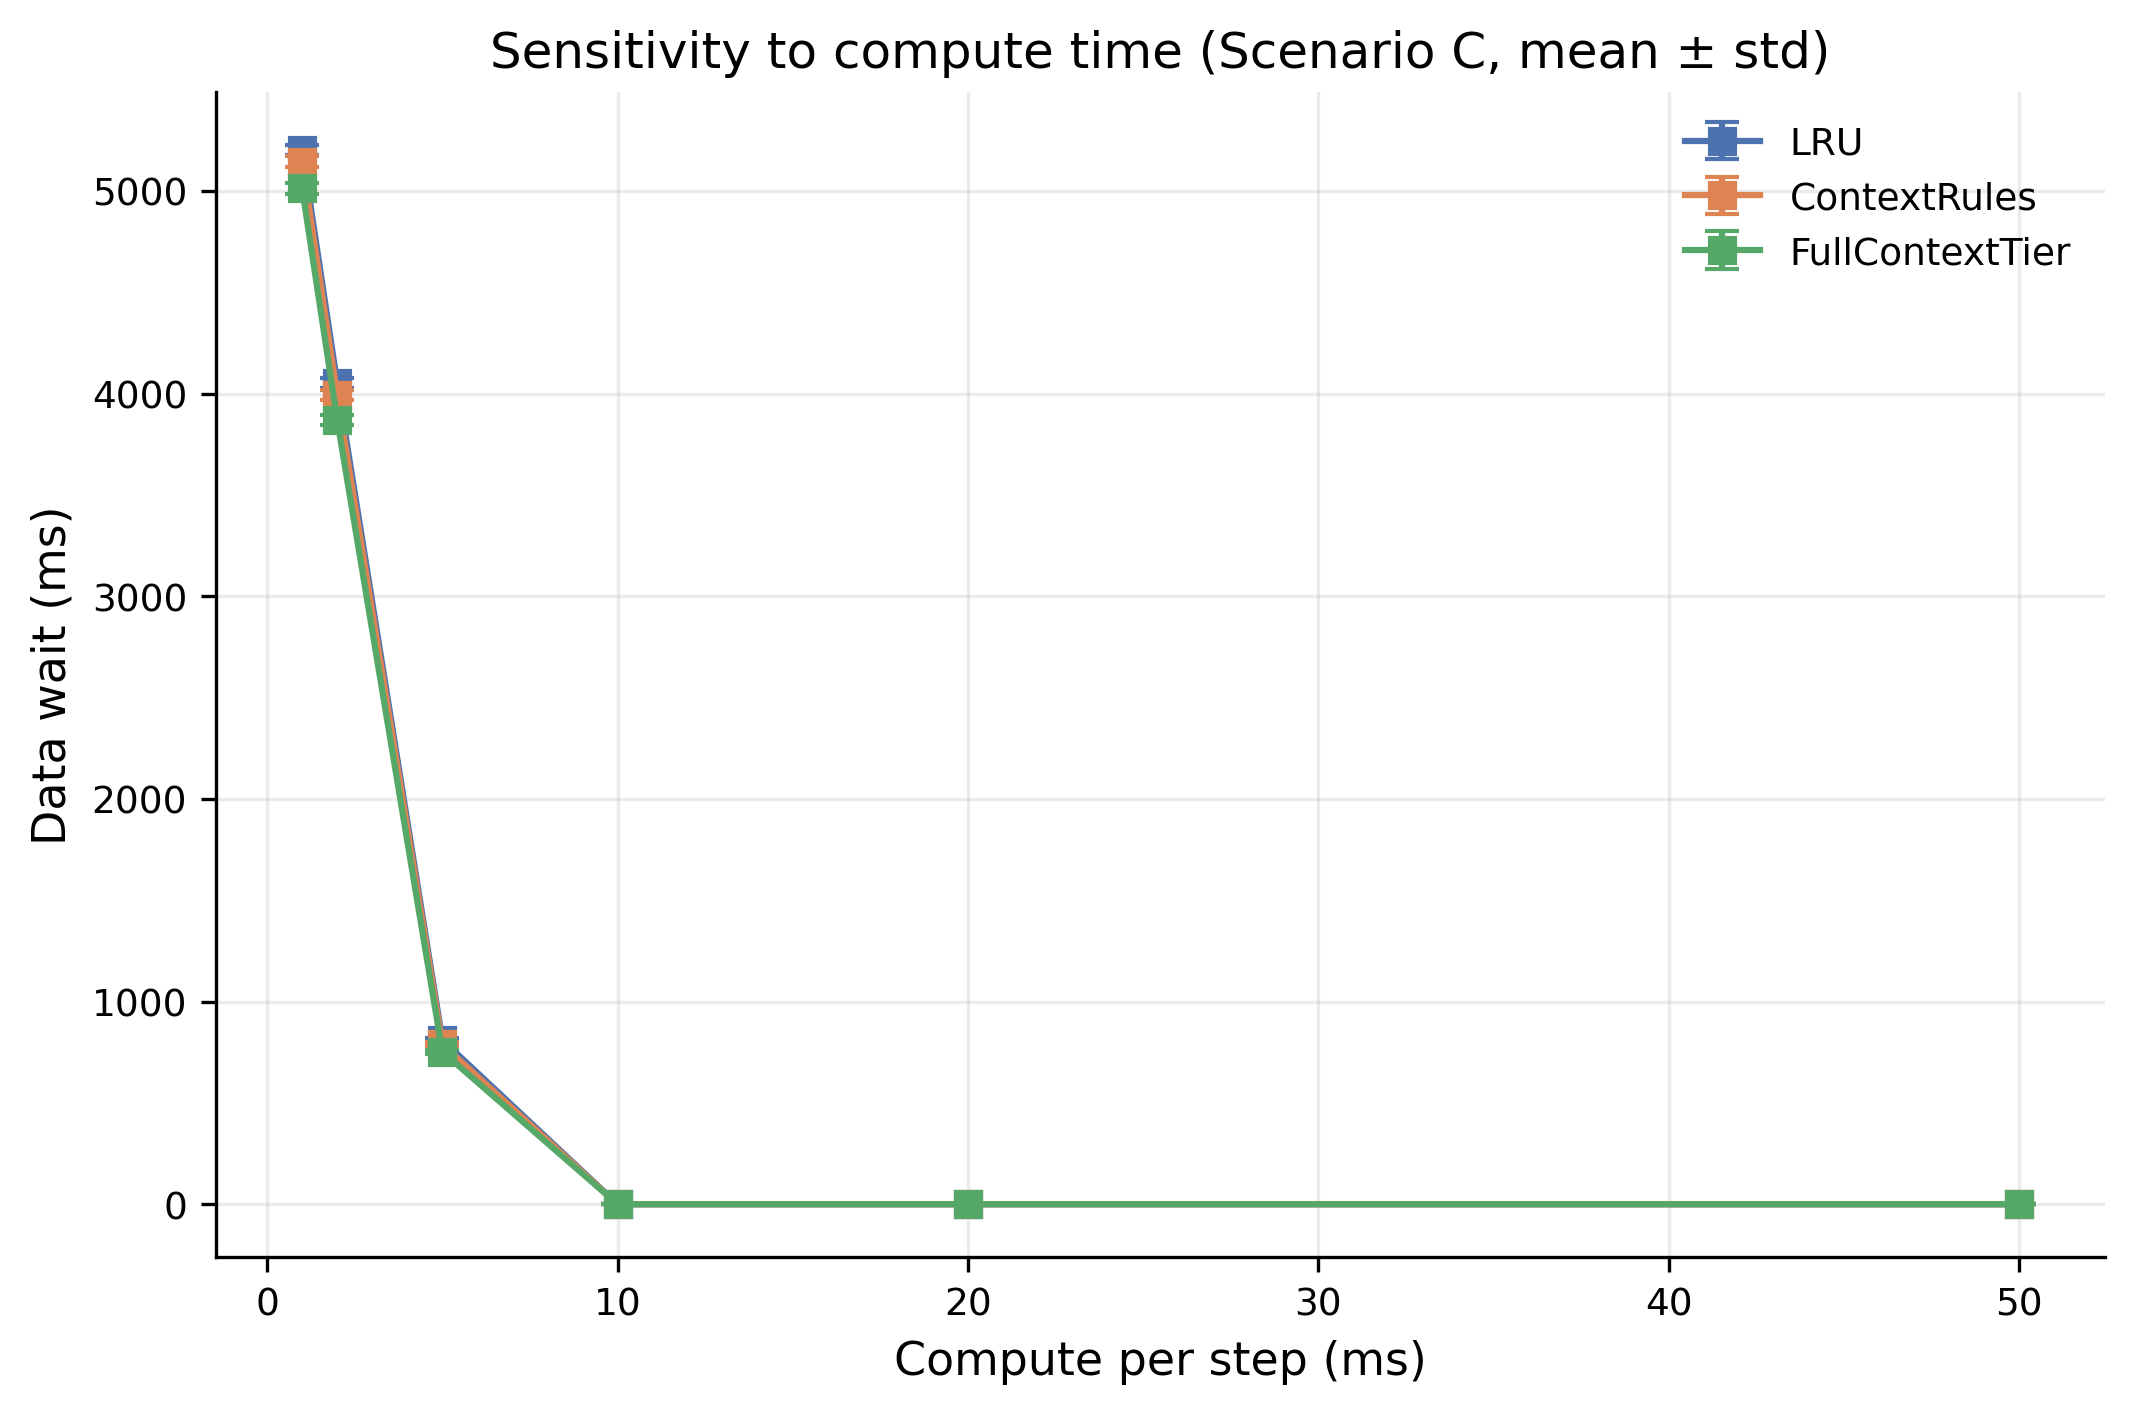
\includegraphics[width=\columnwidth]{compute_sweep.png}
\caption{Compute-per-step sensitivity sweep: Data wait stall (ms) across policies under faster GPU/accelerator execution regimes.}
\label{fig:compute_sweep}
\end{figure}

\begin{figure}[t]
\centering
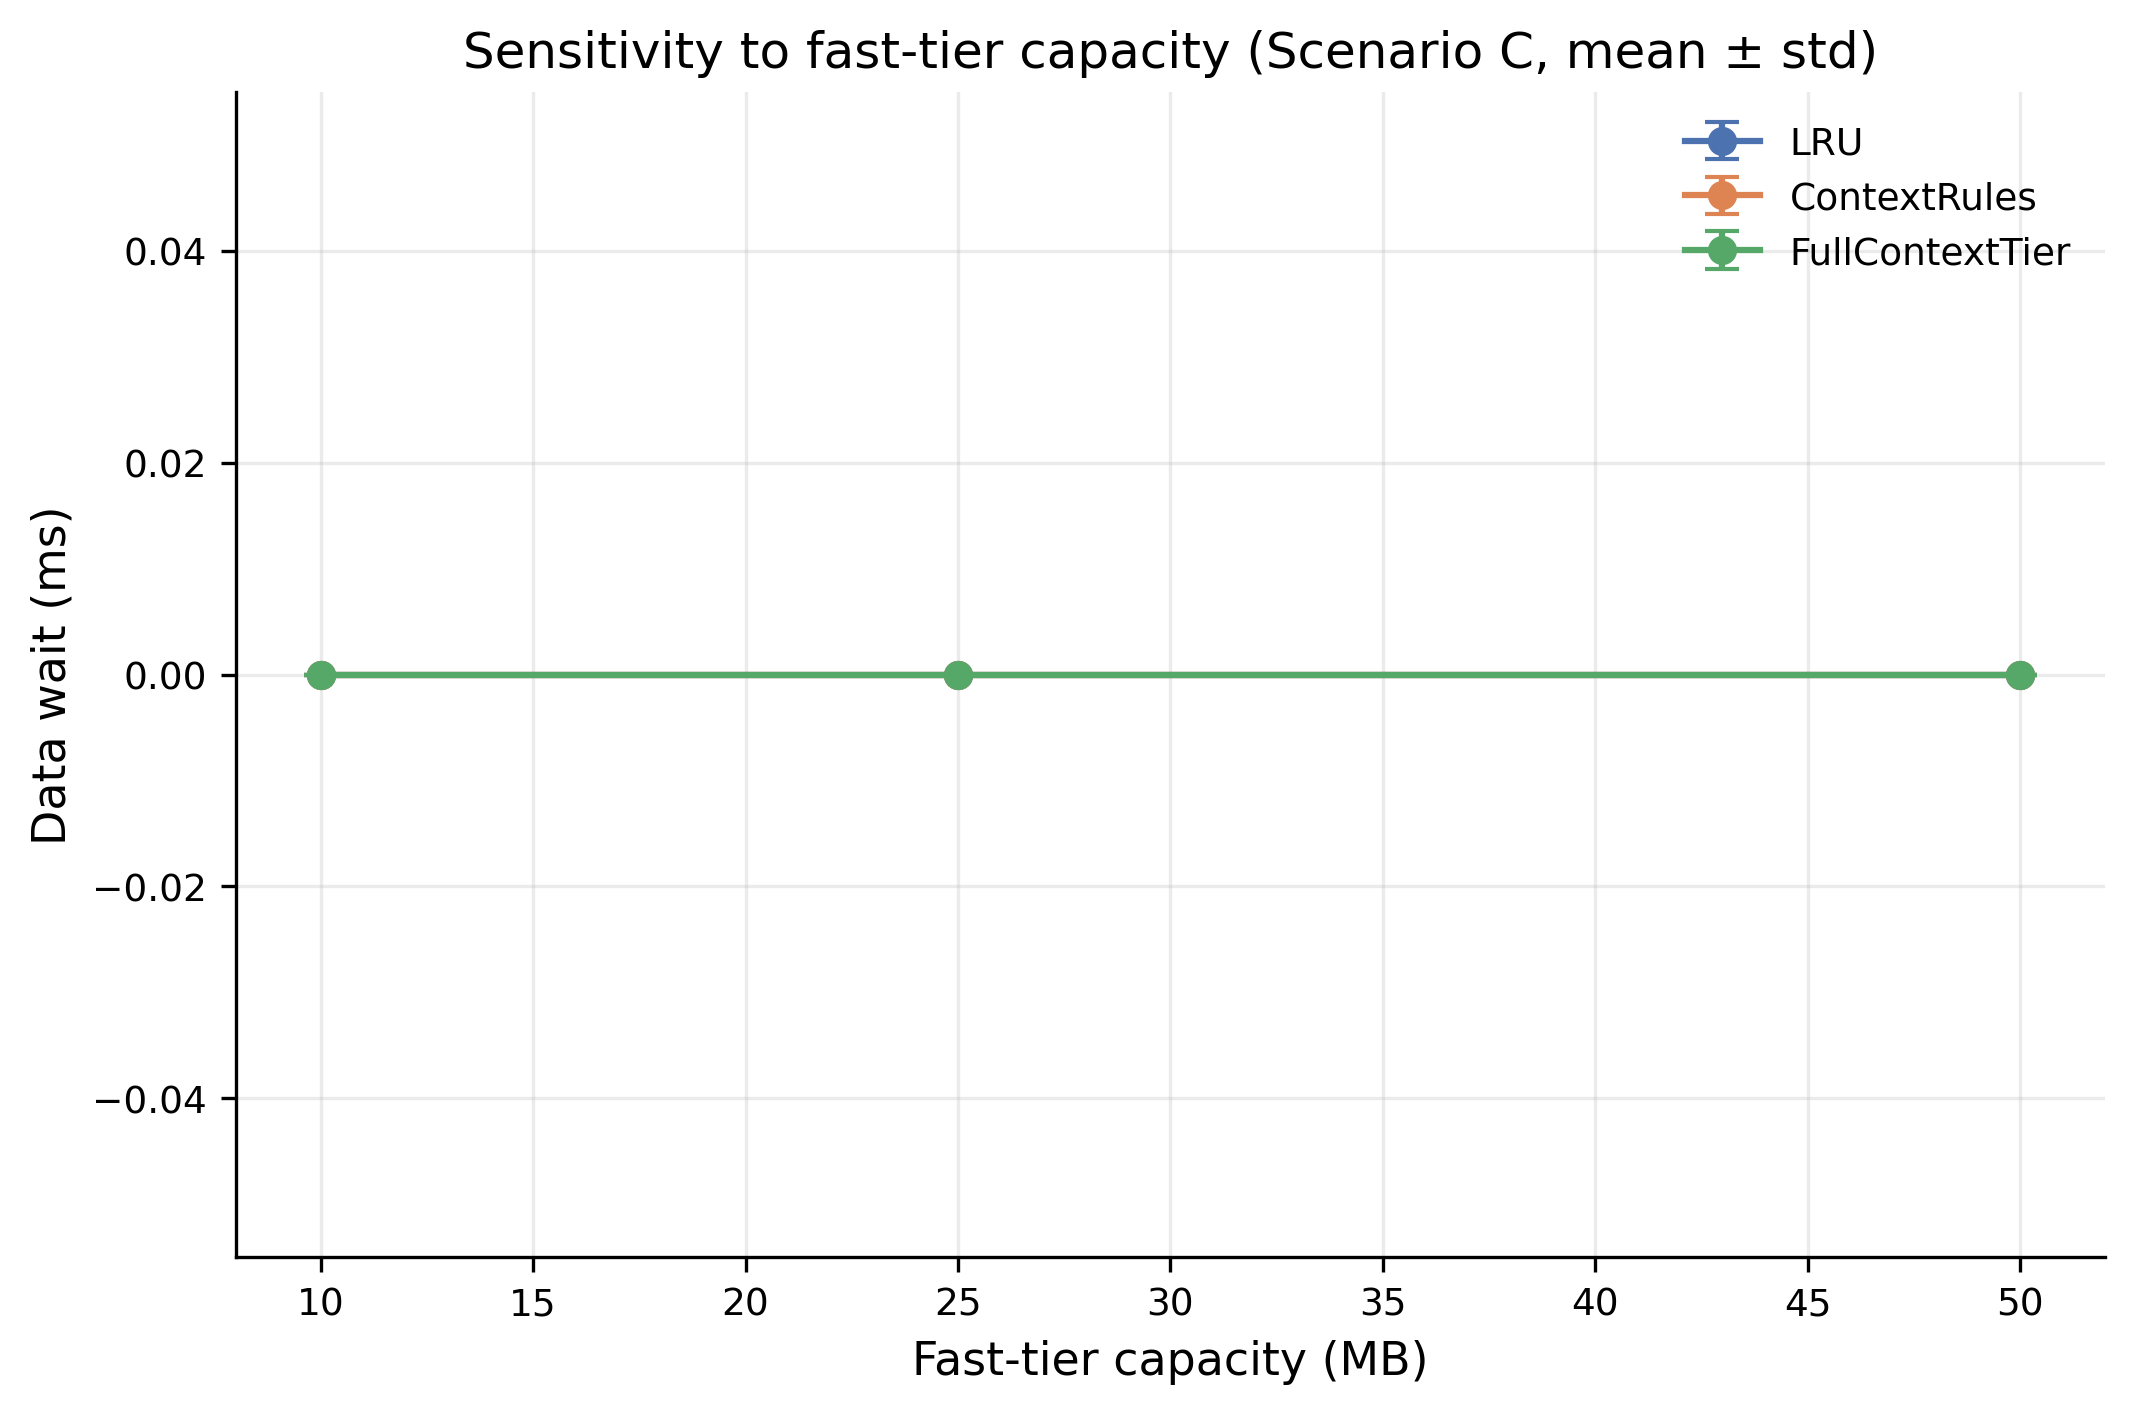
\includegraphics[width=\columnwidth]{capacity_sweep.png}
\caption{Fast-tier RAM capacity sweep: Data wait (ms) as Tier 0 capacity scales from 10~MB to 50~MB.}
\label{fig:capacity_sweep}
\end{figure}

\begin{table}[t]
\centering
\caption{Compute-per-Step Sweep on Scenario C: Data Wait Stall (ms)}
\label{tab:compute_sweep}
\begin{tabular}{lccc}
\toprule
\textbf{Compute Time} & \textbf{LRU Baseline} & \textbf{ContextRules} & \textbf{FullContextTier} \\
\midrule
1 ms & $5,202.47 \pm 24.50$ & $5,144.07 \pm 26.17$ & $\mathbf{5,012.38 \pm 25.65}$ \\
2 ms & $4,050.87 \pm 24.48$ & $3,992.57 \pm 26.13$ & $\mathbf{3,870.15 \pm 25.85}$ \\
5 ms & $810.33 \pm 9.54$ & $788.34 \pm 9.84$ & $\mathbf{752.65 \pm 9.72}$ \\
10 ms & $0.00 \pm 0.00$ & $0.00 \pm 0.00$ & $0.00 \pm 0.00$ \\
20 ms & $0.00 \pm 0.00$ & $0.00 \pm 0.00$ & $0.00 \pm 0.00$ \\
50 ms & $0.00 \pm 0.00$ & $0.00 \pm 0.00$ & $0.00 \pm 0.00$ \\
\bottomrule
\end{tabular}
\end{table}

When deep learning models are executed on modern accelerators (GPUs/TPUs), batch compute times frequently drop to the 1--5~ms range. Fig.~\ref{fig:compute_sweep} and Table~\ref{tab:compute_sweep} evaluate the compute-per-step sensitivity sweep.

As compute overlap decreases, I/O stalls emerge prominently. At 1~ms compute per step:
\begin{itemize}
    \item LRU stalls for 5,202.47~ms.
    \item FullContextTier stalls for only 5,012.38~ms, \textbf{saving 190.09~ms of stall time} [95\% CI: 184.68, 195.66~ms], winning in \textbf{20 out of 20 random seeds}.
    \item At 2~ms, FullContextTier saves 180.73~ms [95\% CI: 175.30, 186.29~ms], winning in 20/20 seeds.
    \item At 5~ms, FullContextTier saves 57.68~ms [95\% CI: 55.48, 59.88~ms], winning in 20/20 seeds.
\end{itemize}
These bootstrap comparisons confirm that under fast accelerator workloads, ContextTier's dynamic tiering delivers statistically significant reductions in I/O stalls.

\subsection{Capacity Sweep and Latency Percentiles}

Fig.~\ref{fig:capacity_sweep} examines the sensitivity of data wait across Tier-0 Fast RAM allocations of 10~MB, 25~MB, and 50~MB. Under the measured CPU step time, all policies maintain zero wait across capacities, confirming that capacity expansion does not alter the compute overlap ceiling.

\begin{figure}[t]
\centering
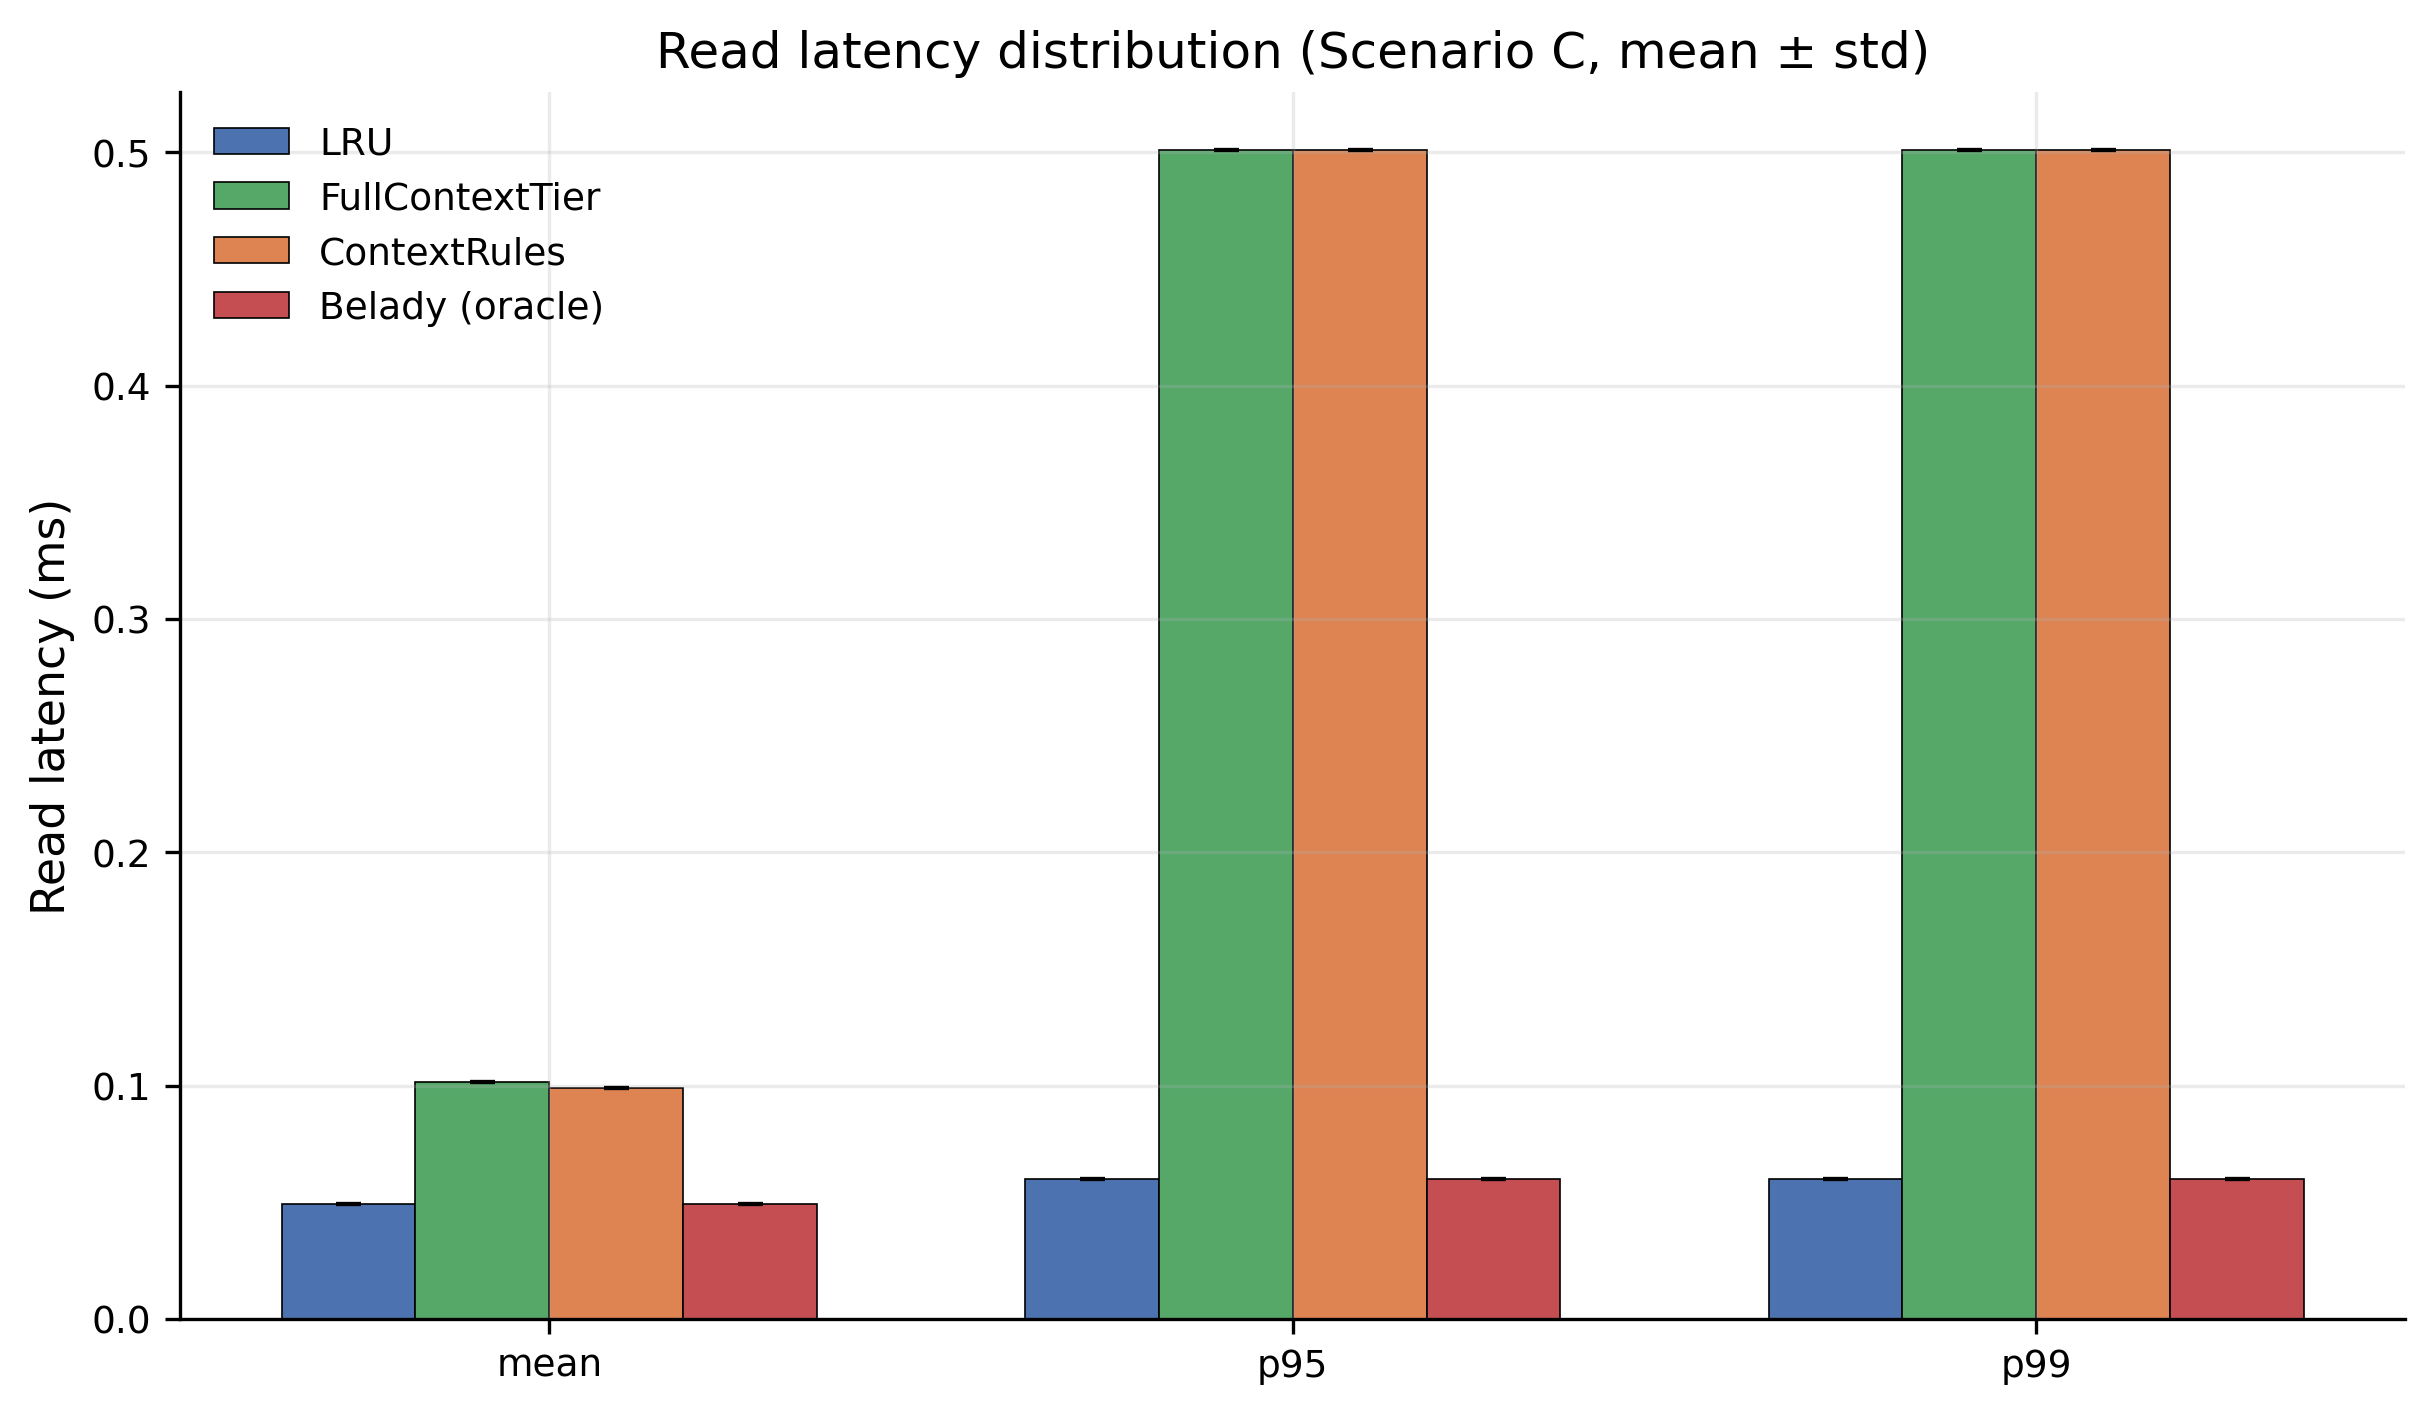
\includegraphics[width=\columnwidth]{latency_percentiles.png}
\caption{Read latency percentiles (Mean, p95, p99 in ms) for representative policies in Scenario C.}
\label{fig:latency_percentiles}
\end{figure}

Fig.~\ref{fig:latency_percentiles} inspects tail read latencies. While LRU achieves a lower p95 latency on validation reads by promoting them to RAM (0.06~ms), FullContextTier deliberately accepts a slightly higher validation latency (0.50~ms in Mid NVMe) in order to protect Tier 0 from eviction, yielding substantially higher overall training throughput.

\section{Discussion and Limitations}
\label{sec:discussion}

\subsection{Why Caching Matters Despite Compute Overlap}
Our findings offer an essential architectural insight: when compute budgets are large, data wait alone cannot evaluate storage policies. In such regimes, caching performance is reflected in \textbf{bus bandwidth consumption} and \textbf{synchronous promotion time}. By preventing validation churn in Tier 0, ContextTier saves 66.4~MB of transfer overhead, preserving bus availability for checkpoint flushes and multi-GPU gradients.

\subsection{Honest Negative Results}
We report two honest negative results:
\begin{enumerate}
    \item \textbf{Speculative Nearest-Neighbor Prefetching:} We initially evaluated speculative prefetching using Word2Vec embedding cosine similarity. Under non-deterministic Scenario C shuffling, speculative prefetching induced severe cache pollution, wasting over 40~MB of bus traffic without reducing stall time. We removed speculative prefetching from the active policy.
    \item \textbf{Linear Function Approximation in RL:} In the RL agent, linear function approximation diverged due to non-stationary feature distributions. We transitioned to a discretized tabular Q-learning representation, which converged reliably across all 12 episodes.
\end{enumerate}

\subsection{Threats to Validity}
This research was evaluated using a calibrated, discrete-event storage emulator on CPU. While hardware transfer speeds (3,000~MB/s RAM, 500~MB/s NVMe, 80~MB/s origin) and batch step times (166.99~ms) were empirically measured, production deployments introduce complex OS page-cache writeback dynamics and multi-tenant NVMe queue contention. Relative policy rankings are validated by real-mode benchmarks (Spearman $\rho = 0.9487$ in Scenario C), but absolute latencies may vary.

\section{Related Work}
\label{sec:related}
\textbf{Deep Learning I/O Prefetching:} NoPFS~\cite{dryden2021clairvoyant} pioneered seed-based prefetching for SGD pipelines, demonstrating massive speedups under uniform shuffling. CoorDL~\cite{coordl2021} and DeepIO~\cite{zhu2018deepio} explored coordinated data loading across distributed training jobs. ContextTier extends this body of work by addressing heterogeneous data roles, multi-tier migration, and non-deterministic state-dependent workloads.

\textbf{Cache Replacement Algorithms:} Classic algorithms such as Belady's MIN~\cite{belady1966study}, LRU, LFU, and ARC~\cite{megiddo2003arc} govern single-tier eviction based on recency and frequency. CacheLib~\cite{cachelib2020} provides multi-tier caching primitives for social workloads. ContextTier differs by integrating reinforcement learning and role inference tailored specifically to deep learning training semantics.

\section{Conclusion}
\label{sec:conclusion}
We presented ContextTier, a context-aware dynamic storage tiering system for deep learning training. By augmenting storage controllers with supervised role classification, Word2Vec sequence modeling, and tabular Q-learning, ContextTier dynamically manages multi-tier hierarchies without requiring oracle true types. Across 20 independent seeds on CIFAR-10 workloads, ContextTier isolates validation bursts to Mid NVMe, saving 63.6~MB of bus bandwidth over standard LRU in 3 epochs, reduces data stall by 190.1~ms under fast compute regimes, and maximizes overall training throughput.

\bibliographystyle{IEEEtran}
\bibliography{references}

\end{document}
